\chapter{Solution approach}

% ~~~~~~~~~~~~~~~~~~~~~~~~~~~~~~~~~~~~~~~~~~~~~~~~~~~~~~~~~~~~~~~~~~~~~~~~~~~~~~~~~~~~~~~~~~~~~~~~~~~~~~~~~~~
\section{Baseline solution}

\begin{itemize}
    \item Adapt existing simple indicators to detect bottlenecks.
        All the indicators consider the relationship between the processing times of jobs on the machines
        and the total (or idle) time.
        
        This idea is still applicable on the \ac{rcpsp}. However, given that the machine load can be variable
        through time, a binary \enquote{processing-idle} differentiation between machine states does not
        provide a sufficient machine-load indication.

        Figure \ref{fig:MachineLoad} illustrates the difference between the variability of the load
        of a Job Shop machine (subfigure \ref{fig:MachineLoad:JS}) and that of a \ac{rcpsp}
        (subfigure \ref{fig:MachineLoad:RCPSP}).
        \todo{Edit RCPSP image: change the second pistachio job to better convey the message of variable load}

    \begin{figure}[t]
      \centering

      \subfloat[Job Shop]{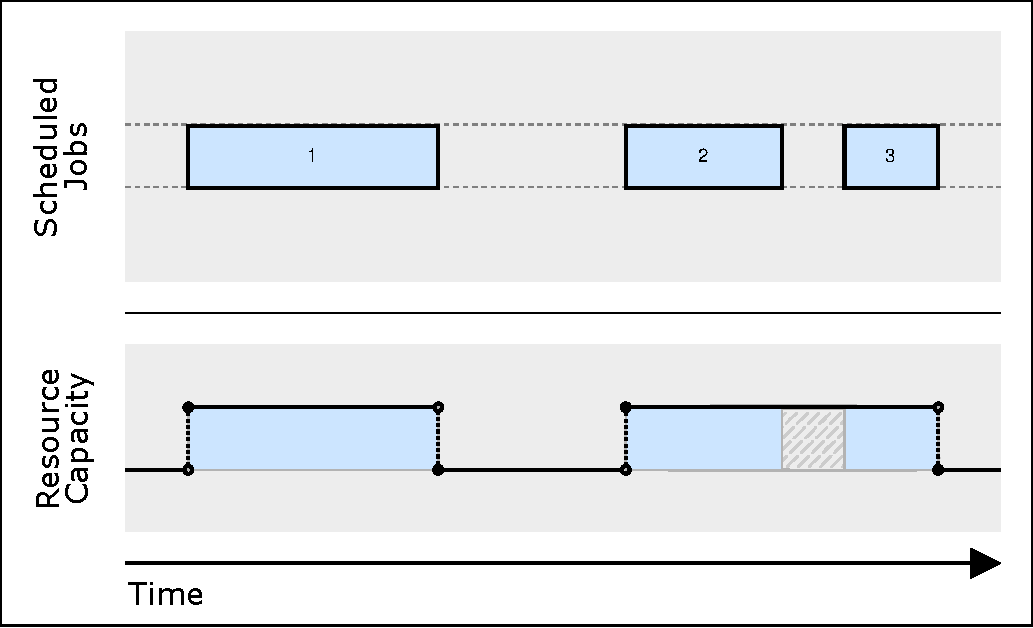
\includegraphics[width=0.7\textwidth]{img/Capacities-JobShop.pdf}\label{fig:MachineLoad:JS}}
      \\
      \subfloat[RCPSP]{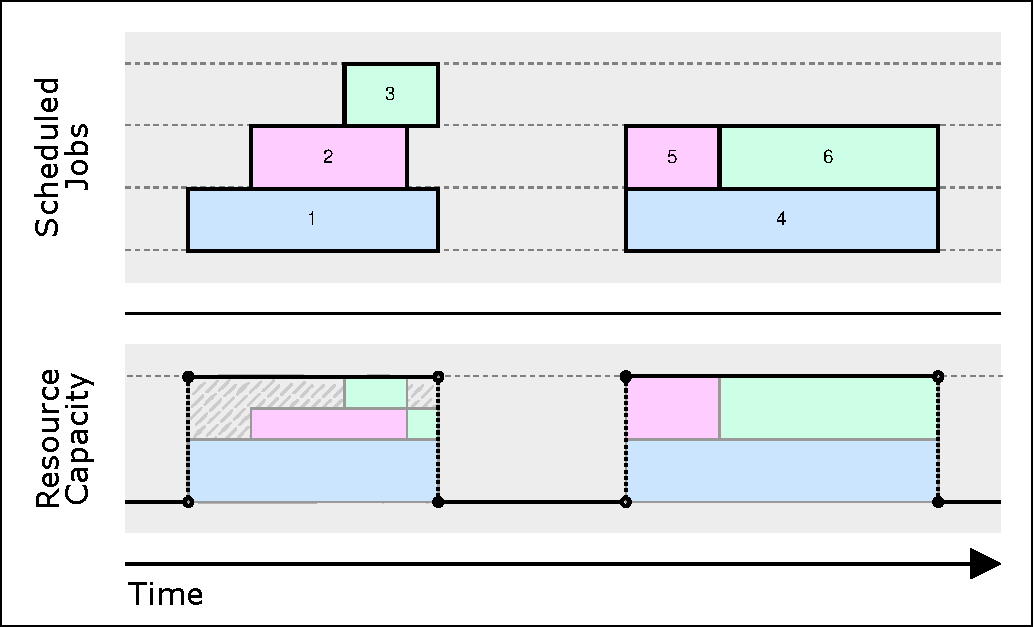
\includegraphics[width=0.7\textwidth]{img/Capacities-RCPSP.pdf}\label{fig:MachineLoad:RCPSP}}

      \caption{Caption.}
      \label{fig:MachineLoad}
    \end{figure}

    We adapt \ac{mw}, \ac{mur}, and \ac{auad} indicators (defined in \todo{ref Related works}) respectively as follows:
    \begin{itemize}
        \item \ac{mrw}
        $$
        \indMRW{k} = \sum_{\substack{j \;:\; \text{$j$ consumes $k$}}} p_j \; r_{jk}
        $$

        \item \ac{mrur}
        $$
        \indMRUR{k} = \frac{\indMRW{k}}{R_k \; (\max_{j \;:\; \text{$j$ consumes $k$}} C_j - \min_{j \;:\; \text{$j$ consumes $k$}} S_j)}
        $$

        \item \ac{auac} \todo{this might be a bit harder}
        $$
        \indAUAC{k} = \begin{cases}
            \frac{\sum_{a \in A_k} \text{consumption in $a$}}{\abs{A_k}} & \dots \text{consumption} \\
            \frac{\sum_{a \in A_k} (\text{consumption in $a$}) / (\text{capacity} \cdot \abs{a}))}{\abs{A_k}} & \dots \text{consumption to capacity ratio} \\
            \frac{\sum_{a \in A_k} (\text{consumption in $a$}) / (\text{capacity}))}{\abs{A_k}} & \dots \text{consumption to capacity ratio times the period length}
            \end{cases}
        $$
    \end{itemize}

    \item Try to find alternative schedule based on the found bottlenecks
    \begin{itemize}
        \item Combinatorial heuristics?
        \item Simplified optimization?
    \end{itemize}
\end{itemize}

% ~~~~~~~~~~~~~~~~~~~~~~~~~~~~~~~~~~~~~~~~~~~~~~~~~~~~~~~~~~~~~~~~~~~~~~~~~~~~~~~~~~~~~~~~~~~~~~~~~~~~~~~~~~~
\section{Extended solution}

\begin{itemize}
    \item Come up with a new way of detecting time-variant bottlenecks
        The sum of delays of jobs using this resource - the delays are from the earliest possible completion
        time computed from the model with no resource constraints.

    \item Apply the method to identify bottlenecks
    \item Relax bottlenecks - one by one, combined?
    \item Propose alternative solutions
    \begin{itemize}
        \item Extremal solutions based on some similarity/improvement metrics?
        \item Scalable solution?
    \end{itemize}
\end{itemize}
